\section{Feedforward Neural Networks}
Before we can understand the architecture of a \textbf{feedforward neural network} (FFNN), we first introduce
how we got here.

\subsection{From Logistic Regression to Feedforward NN}
To fit a model to some data distribution, a simple and common approach is to use \textbf{Maximum Likelihood Estimation} (MLE).
\subsubsection{Maximum Likelihood Estimation}
In MLE, we want to estimate the parameters of an assumed probability distribution, given some observed data. For example, if we assume that the data is generated from a Gaussian distribution, we can estimate the mean and variance of that distribution using MLE.

More formally, given a dataset $\boldsymbol{X} = \{\boldsymbol{x}_1, \boldsymbol{x}_2, \ldots, \boldsymbol{x}_N\}$ and a known probability distribution $p_{\text{model}}(\boldsymbol{x}|\boldsymbol{\theta})$
we want to find the parameters $\boldsymbol{\theta}$ that better explain the data.
\begin{equation}
    \label{MLE}
    \boldsymbol{\theta}^* = \arg\max_{\boldsymbol{\theta}} p_{\text{model}}(\boldsymbol{X}|\boldsymbol{\theta})
\end{equation}
Assuming that the data points are independent and identically distributed (i.i.d.), we can express the likelihood as a product of individual probabilities:
\begin{equation*}
    p_{\text{model}}(\boldsymbol{X}|\boldsymbol{\theta}) = \prod_{i=1}^{N} p_{\text{model}}(\boldsymbol{x}_i|\boldsymbol{\theta})
\end{equation*}
To simplify the optimization process, we often take the logarithm of the likelihood function, which transforms the product into a sum:
\begin{equation*}
    \log p_{\text{model}}(\boldsymbol{X}|\boldsymbol{\theta}) = \sum_{i=1}^{N} \log p_{\text{model}}(\boldsymbol{x}_i|\boldsymbol{\theta})
\end{equation*}
We can show that this is equivalent to considering the expected value of the log-likelihood over the empirical (observed) data distribution:
\begin{equation*}
    \log p_{\text{model}}(\boldsymbol{X}|\boldsymbol{\theta}) = N \cdot \mathbb{E}_{\boldsymbol{x} \sim p_{\text{data}}}[\log p_{\text{model}}(\boldsymbol{x}|\boldsymbol{\theta})]
\end{equation*}
where $p_{\text{data}}$ is the empirical distribution of the observed data and $\mathbb{E}_{\boldsymbol{x} \sim p_{\text{data}}}$ denotes the expected value sampled from this distribution.

To find the optimal parameters $\boldsymbol{\theta}^*$, we usually differentiate the log-likelihood with respect to $\boldsymbol{\theta}$ and set it
to zero. We can then resolve the resulting equation to find the optimal parameters.

The equation \ref{MLE} can also be extended to the case of conditional probability distributions ($p_{\text{model}}(y|\boldsymbol{x}, \boldsymbol{\theta})$) in order to predict a target variable $y$ given an input variable $\boldsymbol{x}$:
\begin{equation*}
    \boldsymbol{\theta}^* = \arg\max_{\boldsymbol{\theta}} p_{\text{model}}(y|\boldsymbol{x}, \boldsymbol{\theta})
\end{equation*}
This is the basis for most supervised learning algorithms, including Linear Regression and Logistic Regression, which simply assume different forms for the conditional probability distribution.
For example, in Logistic Regression, we assume that the conditional probability distribution is given by the logistic function:
\begin{equation}
    \label{Logistic Regression}
    p_{\text{model}}(y=1|\boldsymbol{x}, \boldsymbol{\theta}) = \sigma(\boldsymbol{\theta}^T \boldsymbol{x}) = \frac{1}{1 + e^{-\boldsymbol{\theta}^T \boldsymbol{x}}}
\end{equation}

\subsubsection{Logistic Regression}
Logistic Regression is a linear model used for binary classification tasks.
\begin{comment}
    #TODO: extend here??
\end{comment}
Given the equation \ref{Logistic Regression}, we can observe that the can be seen as a simple Neural Network with a single layer and a sigmoid activation function.

\subsection{Feedforward Neural Networks}
A Feedforward Neural Network (FFNN) is a type of artificial neural network that define a mapping from the input space
to an output space. The learned mapping $f(\boldsymbol{x})$ is defined as a composition of several functions, each representing a layer of the network.
\begin{figure}[H]
    \centering
    \scalebox{0.8}{
        \input{Tikz/FFNN/3-layer-FFNN.tex}
    }
    \caption{Example of a feedforward neural network with three hidden layers.}
    \label{fig:FFNN_example}
\end{figure}

For example, taking in consideration the FFNN architecture shown in the figure \ref{fig:FFNN_example} with three layers, we can express the mapping as follows:
\begin{equation*}
    f(\boldsymbol{x}) = f^{(5)}(f^{(4)}(f^{(3)}(f^{(2)}(f^{(1)}(\boldsymbol{x})))))
\end{equation*}
\begin{itemize}
    \item The first layer $f^{(1)}(\boldsymbol{x})$ is usually referred to as the \textbf{input layer}, each node corresponds to a feature of the input data. Usually no
    computations are performed in this layer, as it simply serves as a conduit for the input data to be fed into the network;
    \item The layers $f^{(2)}$, $f^{(3)}$, and $f^{(4)}$ are called \textbf{hidden layers}, and they perform computations on the input data, applying a linear transformation followed by a non-linear activation function.
    The number of hidden layers and the number of neurons in each hidden layer depend on the architecture of the network and the complexity of the problem being solved.
    \item The last layer $f^{(5)}$ is called the \textbf{output layer}, and it produces the final output of the network. Depending on the type of problem,
    different activation functions can be used (e.g., linear for regression, softmax for classification)
    and different number of neurons can be used (e.g., one for binary classification and regression, one per class for multi-class classification).
\end{itemize}
The function composition can be described by a \textbf{directed acyclic graph} (DAG), where the nodes represent the functions (layers) and the edges represent the flow of data through the network. 
The term "feedforward" comes from the fact that the data flows in one direction, from the input layer to the output layer, without any cycles or loops in the graph.

\subsubsection{Difference from Linear Models}
Linear models are generally very easy to optimize (e.g., closed-form solutions or convex optimization), but they are limited in their expressiveness and cannot capture interactions between features or non-linear relationships in the data.
FFNNs allow to overcome the limitations of linear models by introducing non-linear activation functions and multiple layers of computation.

\subsubsection{How can we improve Linear Models?}
FFNNs are not the only way to improve linear models, but they are one of the most powerful and widely used approaches.
Generally, to boost the performance of linear models, we can apply a non-linear transformation to the input data $\boldsymbol{x} \rightarrow \phi(\boldsymbol{x})$, where $\phi$ is a non-linear function.
We can then apply a linear model to the transformed data $\phi(\boldsymbol{x})$. 
The transformation $\phi$ can be implemented in various ways, such as:
\begin{itemize}
    \item \textbf{Kernel Methods}: map the input data into a high-dimensional feature space (possibly infinite-dimensional) where linear models can be applied.
    This has enough capacity to capture complex relationships in the data, but achieves poor generalization performance for highly variable target functions.
    \item \textbf{Feature Engineering}: manually design and select features that capture relevant information from the input data.
    This was the traditional approach before the rise of deep learning, in particular for computer vision tasks, but it is time-consuming and requires domain expertise.
    \item \textbf{Neural Networks}: learn the transformation $\phi$ from the data itself. This shifts the engineering effort from designing features to designing the architecture of the network,
    but throwhs away the convexity and interpretability. 
\end{itemize}

\subsubsection{Training a FFNN}
To train a Neural Network, we need to optimize the parameters of the network (weights $\boldsymbol{\theta}$) to drive the output of the network $f(\boldsymbol{x}; \boldsymbol{\theta})$
to match the target variable $y$ for a given input $\boldsymbol{x}$.

The training process is nothing different from training any other machine learning model.
We need to define a loss function $\mathcal{L}(f(\boldsymbol{x}; \boldsymbol{\theta}), y)$ that measures the discrepancy between the predicted output and the true target variable.

The largest difference with respect to linear models comes from the fact that most loss functions are non-convex, which removes the guarantee of finding a global minimum and makes the optimization process more challenging.

\subsubsection{Modelling Choices}
When designing a FFNN, we need to make several modelling choices, such as:
\begin{itemize}
    \item \textbf{Cost Function}: the choice of the loss function $\mathcal{L}$ depends on the type of problem we are trying to solve (e.g., regression, classification) and the properties of the data.
    Each function has its own advantages and disadvantages, and the choice can significantly impact the performance of the model.
    \item \textbf{Form of Output}: the function applied in the output layer. Similarly to the cost function, the choice of the output units depends on the type of problem we are trying to solve;
    \item \textbf{Activation Function}: the non-linear function applied in the hidden layers. It's independent from the type of problem we are trying to solve, but it can significantly impact the
    performance of the model and the convergence during training.
    \item \textbf{Architecture}:
    \item \textbf{Optimizer}:
    \item \textbf{Regularizer}:
\end{itemize}

\subsection{Cost Functions}
The porpouse of cost functions is to measure the discrepancy between the predicted output of the network and the true target variable, guiding the parameter optimization process.
Various functions can be defined based on the type of problem.

\subsubsection*{Classification}
\begin{itemize}
    \item \textbf{Categorical Cross-Entropy Loss}: used for multi-class classification problems. It measures the dissimilarity between the predicted
    probability of class $\hat{y}_i$ and the true class label.
    For a single data point, the loss can be expressed as:
    \begin{equation*}
        L(y, \hat{y}) = -\sum_{i=1}^{C} y_i \log(\hat{y}_i)
    \end{equation*}
    \item \textbf{Binary Cross-Entropy Loss}: special case of the categorical cross-entropy loss for binary classification problems.
    For a single data point, the loss can be expressed as:
    \begin{equation*}
        L(y, \hat{y}) = -[y \log(\hat{y}) + (1 - y) \log(1 - \hat{y})]
    \end{equation*}
\end{itemize}

\subsubsection*{Regression}
\begin{itemize}
    \item \textbf{Mean Squared Error (MSE)}: commonly used for regression problems. It measures the average squared difference between the predicted and true values.
    For a single data point, the loss can be expressed as:
    \begin{equation*}
        L(y, \hat{y}) = \frac{1}{2}(y - \hat{y})^2
    \end{equation*}
    It penalizes larger errors more than smaller ones, as the difference is squared. This also makes the loss function convex, which is easier to optimize,
    but it can be very sensitive to outliers in the data, as they can have a disproportionate influence on the overall loss.

    \item \textbf{Mean Absolute Error (MAE)}: similar to MSE but uses the absolute difference instead of the squared difference.
    For a single data point, the loss can be expressed as:
    \begin{equation*}
        L(y, \hat{y}) = |y - \hat{y}|
    \end{equation*}
    This one penalizes large errors less than MSE, making it more robust to outliers in the data.
    \item \textbf{Huber Loss}: combines the properties of MSE and MAE. It behaves like MSE for small errors and like MAE for large errors, providing a balance between sensitivity to outliers and smoothness of the loss function.
    Formally, for a single data point, the loss can be expressed as:
    \begin{equation*}
        L(y, \hat{y}) = \begin{cases}
        \frac{1}{2}(y - \hat{y})^2 & \text{for } |y - \hat{y}| \leq \delta \\
        \delta (|y - \hat{y}| - \frac{1}{2}\delta) & \text{for } |y - \hat{y}| > \delta
        \end{cases}
    \end{equation*}
    where $\delta$ is a hyperparameter that determines the threshold between the MSE and MAE behavior.
\end{itemize}
Many more loss functions exist, and can be tryed out based on the specific problem and data characteristics.

\subsubsection*{Contrastive Learning}
Another branch that is worth mentioning is the one used to train models in a self-supervised way, such as contrastive learning.
As shown in the figure \ref{fig:left}, the idea is to learn a representation of the data that captures the underlying structure and relationships between data points,
that is invariant to certain transformations.

The loss function used in contrastive learning is designed to encourage the model to learn representations that are similar for similar data points and dissimilar for different data points.
A possible loss function for contrastive learning is the \textbf{Noise Contrastive Estimation} (NCE) loss, which can be expressed as follows:
\begin{equation*}
    NCE_{Loss} = -\log \frac{e^{\text{sim}(\boldsymbol{z_i}, \boldsymbol{z_j})}}
    {e^{\text{sim}(\boldsymbol{z_i}, \boldsymbol{z_j})} + \sum_{k=1}^{N} e^{\text{sim}(\boldsymbol{z_i}, \boldsymbol{z_k})}}
\end{equation*}
where $\boldsymbol{z_i}$ and $\boldsymbol{z_j}$ are the representations of two similar data points (anchor and positive), $\boldsymbol{z_k}$ are the representations of all data points (negatives), 
$\text{sim}(\cdot, \cdot)$ is a similarity function (e.g., cosine similarity). 
\begin{figure}[H]
    \centering
    \begin{minipage}{0.45\textwidth}
        \centering
        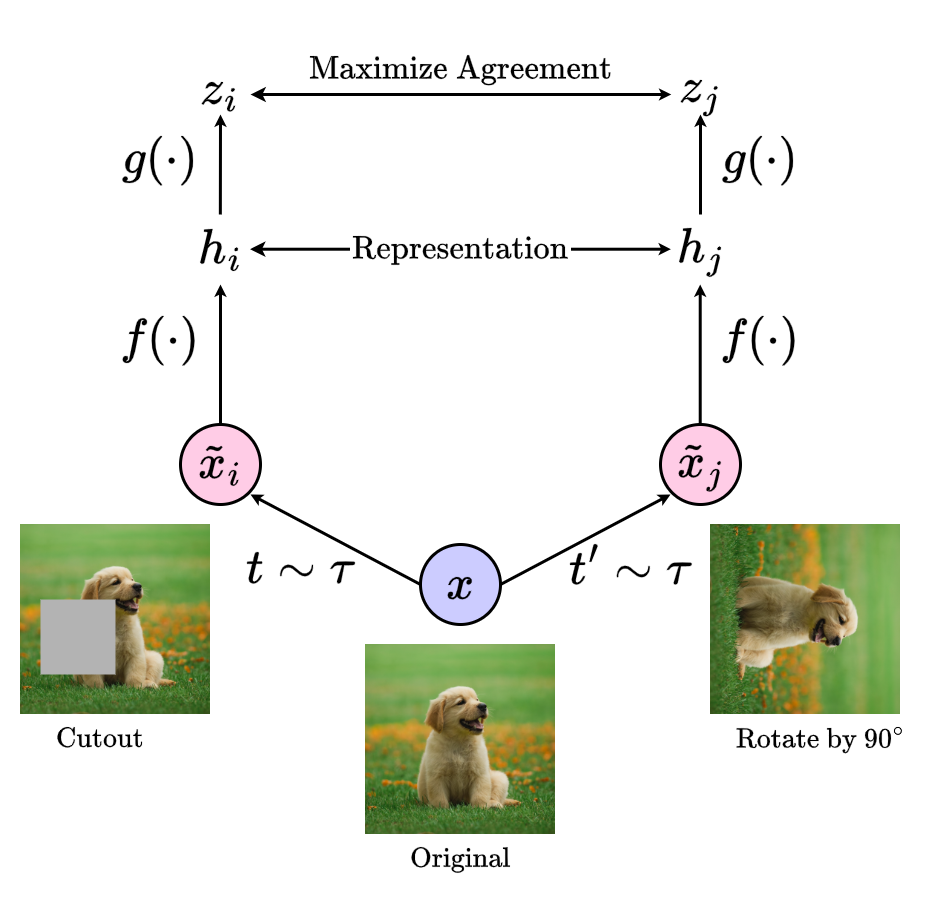
\includegraphics[width=\textwidth]{media/FFNN/contrastive_learning.png}
        \caption{Contrastive learning Model}
        \label{fig:left}
    \end{minipage}
    \hfill
    \begin{minipage}{0.45\textwidth}
        \centering
        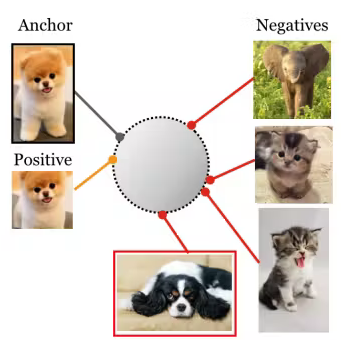
\includegraphics[width=\textwidth]{media/FFNN/contrastive_learning_1.png}
        \caption{Contrastive learning loss function}
        \label{fig:right}
    \end{minipage}
\end{figure}

\subsection{Output Units}
The output units are the last layer of the network, and their choice depends on the type of problem we are trying to solve.
\begin{itemize}
    \item \textbf{Linear Units}: used for regression problems, where the output is simply a linear combination of the inputs.
    \begin{equation*}
        y = \boldsymbol{\theta}^T \boldsymbol{x} + \theta_0
    \end{equation*}
    
    \item \textbf{Softmax Units}: used for multi-class classification problems. They allow to take the unnormalized output of the last hidden layer
    and convert it into a probability distribution over the classes.
    For a given input $\boldsymbol{x}$, the output of the softmax layer can be expressed as:
    \begin{equation*}
        \hat{y}_i = \frac{\exp(z_i)}{\sum_{j=1}^{K} \exp(z_j)}
    \end{equation*}
    where $z_i$ is the output of the last hidden layer for class $i$, and $K$ is the total number of classes.

    This produces a valid probability distribution over the classes, which also handles the multi-class classification case in a natural way.
\end{itemize}
\begin{comment}
    #TODO: maybe more in softmax
\end{comment}

\subsection{Activation Functions}
Hidden units usually use a different activation function than the output units as it is independent from the type of problem we are trying to solve.

What's important to note is that in the choice of activation function it is much more important to 
consider the derivative of the function rather than the function itself, as it is what will be 
used during the backpropagation process to update the weights of the network.
\paragraph{Sigmoid}
Maps the input to a value between 0 and 1, which can be interpreted as a probability. It is defined as:
\begin{figure}[H]
    \centering
    \begin{minipage}{0.45\textwidth}
    \[
    \sigma(x) = \frac{1}{1 + e^{-x}}
    \]
\end{minipage}
\hfill
\begin{minipage}{0.45\textwidth}
    \centering
    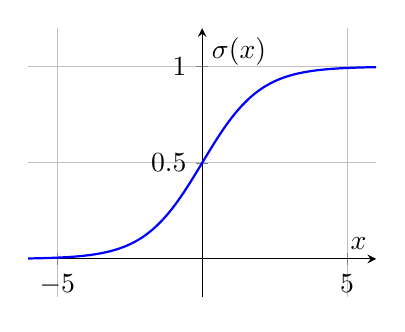
\begin{tikzpicture}[scale=1]
        \begin{axis}[
            xlabel=$x$,
            ylabel=$\sigma(x)$,
            grid=major,
            axis lines=middle,
            xmin=-6, xmax=6,
            ymin=-0.2, ymax=1.2,
            samples=200,
            width=6cm,
            height=5cm
        ]
            \addplot[blue, thick, domain=-6:6] {1/(1+exp(-x))};
        \end{axis}
    \end{tikzpicture}
\end{minipage}

\end{figure}
This function is smooth and differentiable, but it saturates (approaches 0) across most of its domain,
which can lead to the problem of vanishing gradients during training.

\paragraph{Hyperbolic Tangent (tanh)}
Similar to sigmoid but maps the input to a value between -1 and 1. It is defined as:
\begin{figure}[H]
    \centering
    \begin{minipage}{0.45\textwidth}
    \centering
    \[
    \tanh(x) = 2\sigma(2x) - 1 = \frac{e^x - e^{-x}}{e^x + e^{-x}}
    \]
\end{minipage}
\hfill
\begin{minipage}{0.45\textwidth}
    \centering
    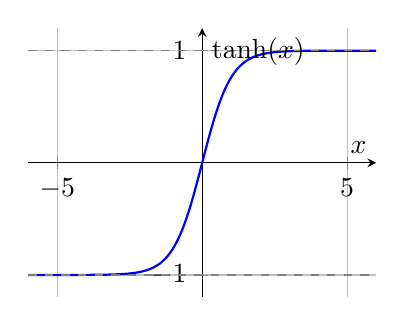
\begin{tikzpicture}[scale=1]
        \begin{axis}[
            xlabel=$x$,
            ylabel=$\tanh(x)$,
            grid=major,
            axis lines=middle,
            xmin=-6, xmax=6,
            ymin=-1.2, ymax=1.2,
            samples=200,
            width=6cm,
            height=5cm
        ]
            \addplot[blue, thick, domain=-6:6] {tanh(x)};
            \addplot[dashed, gray] coordinates {(-6,1) (6,1)};
            \addplot[dashed, gray] coordinates {(-6,-1) (6,-1)};
        \end{axis}
    \end{tikzpicture}
\end{minipage}

\end{figure}
This is better than the sigmoid function as it is zero-centered, which can help with convergence during training,
but it still suffers from the saturation problem for large positive and negative values.

\paragraph{ReLU}
The most commonly used activation function in hidden layers. It is defined as:
\begin{figure}[H]
    \centering
    \begin{minipage}{0.45\textwidth}
    \centering
    \[
    \text{ReLU}(x) = \max(0, x)
    \]
\end{minipage}
\hfill
\begin{minipage}{0.45\textwidth}
    \centering
    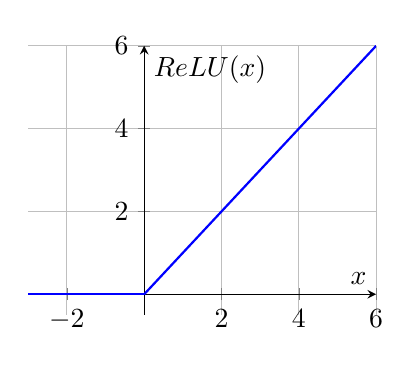
\begin{tikzpicture}[scale=1]
        \begin{axis}[
            xlabel=$x$,
            ylabel=$\text{ReLU}(x)$,
            grid=major,
            axis lines=middle,
            xmin=-3, xmax=6,
            ymin=-0.5, ymax=6,
            samples=200,
            width=6cm,
            height=5cm
        ]
            \addplot[blue, thick, domain=-3:0] {0};
            \addplot[blue, thick, domain=0:6] {x};
        \end{axis}
    \end{tikzpicture}
\end{minipage}

\end{figure}
Born to solve the saturation problem of sigmoid and tanh, the ReLU function is in fact non-saturating for positive values (derivative is 1) which allows for faster convergence during training.

However, this function has still a few negative aspects:
\begin{itemize}
    \item \textbf{Non zero centered output}: similarly to the sigmoid, also the output of the ReLU is non-zero centered;
    \item \textbf{Dying ReLU}: Whenever the input of a neuron is negative, the output is zero, leading to fewer neurons being activated.
    This leads to the "dying ReLU" problem, where neurons can become inactive and only output zero for all inputs, which can hinder learning.
    This usually happens when most of the inputs for a neuron are in the negative range, making the function return 0. Also, the gradients for these neurons will be zero,
    which means that during backpropagation, the weights of these neurons will not be updated, leading to a situation where the neuron is "dead" and cannot recover.
\end{itemize}
Different solutions have been proposed to solve the dying ReLU problem, such as:
\begin{itemize}
    \item \textbf{Stochastic Gradient Descent (SGD)}: the randomness introduced by SGD can help to prevent neurons from dying, as it allows for some updates to the weights even for neurons that are currently inactive.
    \item \textbf{Lower Learning Rates}: using too high learning rates can cause the weights to update too aggressively, possibly leading to weights in the highly negative range;
    \item \textbf{Generalized ReLU}: A family of variants of the ReLU function that introduce a non-zero slope for negative inputs, allowing for a small gradient even when the input is negative.
    Formally, the Generalized ReLU can be expressed as:
    \begin{equation*}
    \text{GReLU}(x) = \begin{cases} x & x \geq 0 \\ \alpha x & x < 0 \end{cases}
    \end{equation*}
    where $\alpha$ is a hyperparameter that controls the slope for negative inputs. Different choices of $\alpha$ lead to different variants of the ReLU function, such as:
    \begin{itemize}
        \item \textbf{Leaky ReLU}: a variant of ReLU that allows a small, non-zero gradient for negative values. It is defined as:
        \begin{figure}[H]
            \centering
            \begin{minipage}{0.45\textwidth}
    \centering
    \[
    \text{Leaky ReLU}(x) = \begin{cases} \alpha x & x < 0 \\ x & x \geq 0 \end{cases}
    \]
    where $\alpha = 0.1$
\end{minipage}
\hfill
\begin{minipage}{0.45\textwidth}
    \centering
    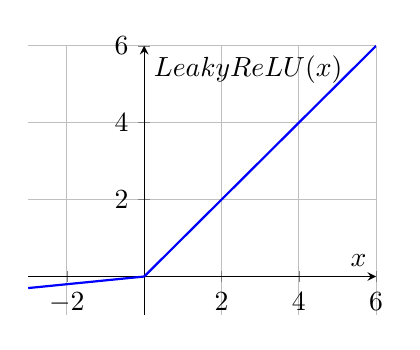
\begin{tikzpicture}[scale=1]
        \begin{axis}[
            xlabel=$x$,
            ylabel=$\text{Leaky ReLU}(x)$,
            grid=major,
            axis lines=middle,
            xmin=-3, xmax=6,
            ymin=-1, ymax=6,
            samples=200,
            width=6cm,
            height=5cm
        ]
            \addplot[blue, thick, domain=-3:0] {0.1*x};
            \addplot[blue, thick, domain=0:6] {x};
        \end{axis}
    \end{tikzpicture}
\end{minipage}

        \end{figure}
        \item \textbf{Parametric ReLU (PReLU)}: where $\alpha$ is a learnable parameter that is updated during training;
        \item \textbf{Randomized ReLU (RReLU)}: where $\alpha$ is randomly sampled from a uniform distribution during training, and fixed to a value during testing;
        \item \textbf{Exponential Linear Unit (ELU)}: where the function is defined as:
        \begin{equation*}
            \text{ELU}(x) = \begin{cases} x & x \geq 0 \\ \alpha (e^x - 1) & x < 0 \end{cases}
        \end{equation*}
        This has all the benefits of ReLU while avoiding the dying ReLU problem, but requires more computational resources due to the exponential function.
    \end{itemize}
\end{itemize}
All this proposed solutions have the common property of being monotonic for positive values. Recently,
non-monotonic activation functions have been proposed, such as:
\begin{itemize}
    \item \textbf{Swish}: defined as $f(x) = x \cdot \sigma(x)$, where $\sigma(x)$ is the sigmoid function.
    The resulting function is non-monotonic and smooth everywhere, which has shown to perform better than ReLU in some cases, but 
    it is more computationally expensive due to the sigmoid function.
    \item \textbf{GelU}: defined as $f(x) = x \cdot \Phi(x)$, where $\Phi(x)$ is an approximation of the cumulative 
    distribution function of the standard normal distribution.
    This function integrates the properties of ReLU and regularizations techniques, such as dropout and zoneout.
\end{itemize}

\subsection{Architectures}
When designing a FFNN, we need to make several choices regarding the architecture of the network, such as:
\begin{itemize}
    \item \textbf{Number of Layers}: how deep should the network be?
    \item \textbf{Number of Neurons per Layer}: how many neurons should each layer have?
    \item \textbf{Expressiveness of the Network}: how complex should the network be to capture the underlying structure of the data?
\end{itemize}
We know that a 2-layer Neural network are universal function approximators, which means that they can approximate any continuous 
function to an arbitrary degree of accuracy, given enough neurons in the hidden layer.
This implies that we could use a shallow network with a single hidden layer, by increasing the number of neurons in that layer (wide network).

However, in practice, it's not guaranteed that our training algorithm will find the optimal parameters that allow the network to approximate the target function, 
as we have to take into consideration the problems in optimization and generalization.
It has been shown that deeper networks can generally capture more complex functions and achieve better generalization performance than shallower networks.

However, increasing the depth of the network is not always the best solution.
Other approaches instead focused on architecutral design choices rather than depth. In particular, this idea was first explored in the context of Convolutional
Neural Networks (CNNs), where the use of convolutional layers allows to get better performance with fewer parameters compared to FFNNs with fully connected layers.

\subsection{Optimization}
To train a FFNN, we need to optimize the parameters of the network to minimize the loss function. 
This is usually done using gradient-based optimization algorithms, such as gradient descent and its variants. 

These algorithms are based on the idea of iteratively updating the parameters of the network in the direction of the steepest descent
of the loss function, which is given by the negative of the gradient of the loss function with respect to the parameters.
To better understand this, let's first introduce the concept of gradients.

\subsubsection{Gradients}
Gradients are a vector of partial derivatives that indicate the \textbf{direction} and \textbf{magnitude} of the \textbf{steepest ascent} of a function. 
Given the loss function $\mathcal{L}(\boldsymbol{W})$, the gradient with respect to the parameters $w_i$ is given by:
\begin{equation*}
    \nabla_{w_i} \mathcal{L} = \left[ \frac{\partial \mathcal{L}}{\partial w_1}, \frac{\partial \mathcal{L}}{\partial w_2}, \ldots, \frac{\partial \mathcal{L}}{\partial w_N} \right]
\end{equation*}
Each component of the gradient vector $\frac{\partial \mathcal{L}}{\partial w_i}$ measures the rate of change of the loss function 
with respect to each parameter.
\begin{figure}[H]
    \centering
    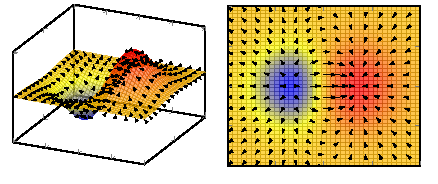
\includegraphics[width=\textwidth]{media/FFNN/partial_derivatives.pdf}
    \caption{Visualization of derivatives and gradients.}
\end{figure}
If we move on the opposite side of the gradients, we will be moving in the direction of the \textbf{steepest descent} of the loss function.
This way, these algorithms can iteratively explore the parameter space to find the optimal parameters that minimize the loss function.
\begin{figure}[H]
    \centering
    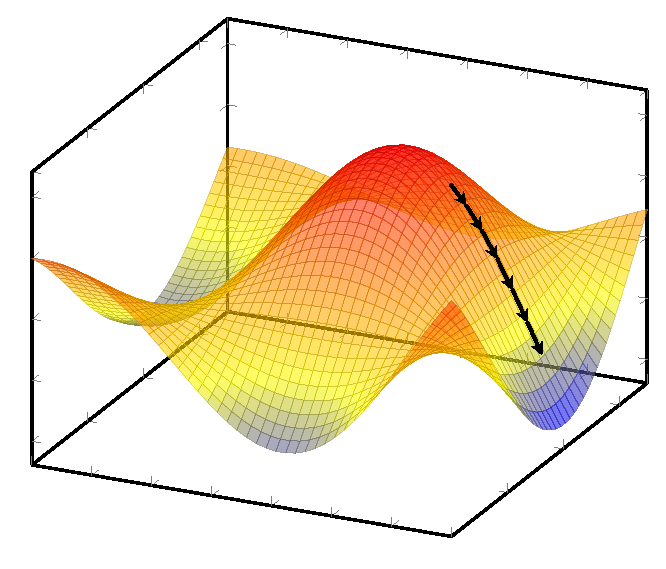
\includegraphics[width=\textwidth]{media/FFNN/gradient-descent.pdf}
    \caption{Visualization of Gradient Descent.}
\end{figure}

\subsubsection{Problems with gradients}
By now we know that in neural networks, the loss function is usually non-convex, which means that it can have multiple local minima and saddle points.

\paragraph{Local minima} Local minima are points in the parameter space where the loss function has a lower value than in the surrounding area,
but it is not the global minimum. This can lead to suboptimal performance of the model.

\paragraph{Saddle points} Similarly, saddle points are points in the parameter space where the loss function has a gradient of zero,
but does not correspond to a local minimum.

Both local minima and saddle points are issues that can arise during the optimization process. Altough they can lead to suboptimal performance,
there are still other issues regarding optimization, that are much more important.

\subsubsection{Gradient Descent}
Gradient Descent is an optimization algorithm used to minimize the loss function by iteratively updating the parameters of the model
in the direction of the negative gradient of the loss function with respect to the parameters.

In the general case, we can express the update rule for the parameters $\boldsymbol{\theta}$ as follows:
\begin{equation*}
    \nabla \leftarrow  \frac{1}{N} \nabla_{\boldsymbol{\theta}} \sum_{i=1}^{N} \mathcal{L}(f(\boldsymbol{x}_i; \boldsymbol{\theta}), y_i)
\end{equation*}
\begin{equation*}
    \boldsymbol{\theta} \leftarrow \boldsymbol{\theta} - \eta \nabla
\end{equation*}
where $\eta$ is the learning rate, which controls the step size of the updates and some parameter initialization is required to start the optimization process.


However, computing the gradient over the entire dataset can be computationally expensive, especially for large datasets.

\subsubsection{Stochastic Gradient Descent}
Stochastic Gradient Descent (SGD) is a variant of gradient descent that updates the parameters using only a single training example at a time, allowing for faster updates and convergence.
The update rule for SGD can be expressed as follows:
\begin{equation*}
    \nabla \leftarrow  \nabla_{\boldsymbol{\theta}} \mathcal{L}(f(\boldsymbol{x}_i; \boldsymbol{\theta}), y_i)
\end{equation*}
\begin{equation*}
    \boldsymbol{\theta} \leftarrow \boldsymbol{\theta} - \eta \nabla
\end{equation*}
where $i$ is randomly selected from the training dataset at each iteration.
This allows for faster updates and convergence, but it can also introduce more noise into the optimization process, which can lead to a less stable convergence.

\subsection{Backpropagation}
The perceptron learning algorithm (see \ref{perceptron-training}) is not suitable for training FFNNs,
as it requires to compute the difference between the predicted output and the ground truth for each training example.
This is not possible for FFNNs, as in fact for hidden layers we don't have access to the true output, and we need to compute 
the error based on the output of the network and the true target variable.

To solve this problem, we can use the \textbf{Stochastic Gradient Descent} (SGD) algorithm, in combination with the \textbf{backpropagation} algorithm, 
which allows to efficiently compute the gradients of the loss function with respect to the parameters of the network.
\subsubsection{Idea behind Backpropagation}
Before backpropagation, a few ideas were proposed to learn the weights inside a FFNN:
\begin{itemize}
    \item \textbf{Randomly perturb the weights}: randomly perturb one weight at a time and check
    if the loss function decreases. This is inefficient and does not scale well with the number of parameters in the network.
    \item \textbf{Parallel Perturbation}: randomly perturb all the weights at the same time and check if the loss function decreases.
    This doesn't help at all, as we would need many perturbations to get a good estimate of the gradient;
    \item \textbf{Perturb the activations}: randomly perturb the activations of the hidden layers and check if the loss function decreases. 
    This is more efficient than perturbing the weights, as we have fewer activations than weights, but it still does not scale well with the number of parameters in the network.
\end{itemize}
From the last idea, the backpropagation algorithm was born, which instead measure how the loss function changes with respect to the activations of the hidden layers.

\subsubsection{The algorithm}
The backpropagation algorithm, introduced in the section \ref{introduction-backpropagation}, consists of three main steps:
\begin{itemize}
    \item \textbf{Forward Pass}: compute the output of the network for a given input $\boldsymbol{x}$ and the current parameters $\boldsymbol{\theta}$;
    \item \textbf{Error Computation}: compute the error at the output layer by comparing the predicted output with the true target variable $y$;
    \item \textbf{Backward Pass}: propagate the error signal back through the network, allowing to update the parameters of the network using the computed gradients.
\end{itemize}
As said before, we cannot know from the training data what the expected output of the hidden units should be, but we can compute how
the error changes with respect to the change in the hidden units.

\subsubsection{Single Neuron Case}
Let's first consider a neural network with just one neuron in each layer.
After performing the forward pass, we can express the output of the network as follows:
\begin{equation*}
    a^{(L)} = \sigma(z^{(L)}) = \sigma(w^{(L)} a^{(L-1)} + b^{(L)})
\end{equation*}
where $a^{(L)}$ is the output of the last layer, $\sigma$ is a non-linear activation function, 
$w^{(L)}$ and $b^{(L)}$ are respectively the weight and bias of the last layer, and $a^{(L-1)}$ is the output of the previous layer.

Our goal is to understand how a small change in the parameters $w^{(l)}$ will affect the loss function $\mathcal{L}$.
When computing this, we need to consider the chain of dependencies between the parameters and the loss function:
\begin{itemize}
    \item How a change in $w^{(l)}$ affects the output of the layer $z^{(l)}$;
    \item How a change in $z^{(l)}$ affects the output of the layer $a^{(l)}$;
    \item How a change in $a^{(l)}$ affects the loss function $\mathcal{L}$.
\end{itemize}
This is where the chain rule of calculus comes into play, allowing us to compute the gradient of the 
loss function with respect to the parameters by multiplying the gradients along the chain of dependencies.

Formally, we can express the gradient of the loss function with respect to the parameters $w^{(l)}$ as follows:
\begin{equation*}
    \frac{\partial \mathcal{L}}{\partial w^{(l)}} = \frac{\partial z^{(l)}}{\partial w^{(l)}} \cdot \frac{\partial a^{(l)}}{\partial z^{(l)}} \cdot \frac{\partial \mathcal{L}}{\partial a^{(l)}}
\end{equation*}
where respectively:
\begin{itemize}
    \item $\frac{\partial z^{(l)}}{\partial w^{(l)}}$ measures how a small change in the weight $w^{(l)}$ affects the output of the layer $z^{(l)}$;
    \item $\frac{\partial a^{(l)}}{\partial z^{(l)}}$ measures how a small change in the output of the layer $z^{(l)}$ affects the output of the activation function $a^{(l)}$;
    \item $\frac{\partial \mathcal{L}}{\partial a^{(l)}}$ measures how a small change in the output of the activation function $a^{(l)}$ affects the loss function $\mathcal{L}$.
\end{itemize}
The process can be extended to deeper layers. In those cases, we need to consider the chain of dependencies from the parameter we want to update
to the output of the network, computing the gradients along the way using the chain rule of calculus.
\begin{figure}[H]
    \centering
    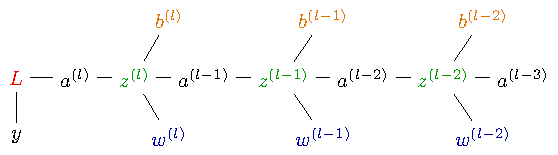
\includegraphics[width=\textwidth]{media/FFNN/dependencies.pdf}
    \caption{Dependency chain for a parameter in a deep network.}
\end{figure}
Taking in consideration the architecture shown in the figure above, we can express the derivative of the loss function with respect to a parameter $w^{(l-1)}$ in a deeper layer as follows:
\begin{equation*}
    \frac{\partial \mathcal{L}}{\partial w^{(l-1)}} = \frac{\partial z^{(l-1)}}{\partial w^{(l-1)}} \cdot \frac{\partial a^{(l-1)}}{\partial z^{(l-1)}} \cdot \underbrace{\frac{\partial z^{(l)}}{\partial a^{(l-1)}} \cdot \frac{\partial a^{(l)}}{\partial z^{(l)}} \cdot \frac{\partial \mathcal{L}}{\partial a^{(l)}}}_{\frac{\partial \mathcal{L}}{\partial a^{(l-1)}}}
\end{equation*}
\subsubsection{General Case}
The general case of backpropagation doesn't differ much from the single neuron case. We simply have to consider all the possible
way in which a change in a parameter can affect the loss function, and compute the gradients accordingly using the chain rule of calculus.

To take into account the fact that each layer can have multiple neurons, we also need to update the notation. Since each connection in the network has its own weight,
we represent with $w_{ij}^{(l)}$ the weight connecting the $j$-th neuron in layer $l-1$ to the $i$-th neuron in layer $l$.

The weighted sum for the $i$-th neuron in layer $l$ can be expressed as follows:
\begin{equation*}
    z_i^{(l)} = \sum_{j} w_{ij}^{(l)} a_j^{(l-1)} + b_i^{(l)}
\end{equation*}
where $a_j^{(l-1)}$ is the output of the $j$-th neuron in the previous layer, and $b_i^{(l)}$ is the bias term for the $i$-th neuron in layer $l$.

When we consider the output layer neurons, the chain of dependencies remains the same as in the single neuron case, as each output neuron is directly connected to the loss function.
\begin{equation*}
    \frac{\partial \mathcal{L}}{\partial w_{ij}^{(L)}} = \frac{\partial z_i^{(L)}}{\partial w_{ij}^{(L)}} \cdot \frac{\partial a_i^{(L)}}{\partial z_i^{(L)}} \cdot \frac{\partial \mathcal{L}}{\partial a_i^{(L)}}
\end{equation*}

For the hidden layer neurons, we instead need to consider all the possible paths from the parameter we want to update to the output layer, and compute the gradients accordingly.
\begin{figure}[H]
    \centering
    \scalebox{0.5}{\input{Tikz/FFNN/back-prop-focus.tex}}
    \caption{Dependency chain for a parameter feeding into $h_2$.}
    \label{fig:backpropagation_output}
\end{figure}
\begin{equation*}
    \frac{\partial \mathcal{L}}{\partial a_j^{(l-1)}} = \sum_{i} \frac{\partial z_i^{(l)}}{\partial a_j^{(l-1)}} \cdot \frac{\partial a_i^{(l)}}{\partial z_i^{(l)}} \cdot \frac{\partial \mathcal{L}}{\partial a_i^{(l)}}
\end{equation*}



